\documentclass[12pt]{article}


\usepackage[utf8]{inputenc} % allow utf-8 input
\usepackage[T1]{fontenc}    % use 8-bit T1 fonts
\usepackage{hyperref}       % hyperlinks
\usepackage{url}            % simple URL typesetting
\usepackage{booktabs}       % professional-quality tables
\usepackage{amsfonts}       % blackboard math symbols
\usepackage{nicefrac}       % compact symbols for 1/2, etc.
\usepackage{microtype}      % microtypography




\usepackage[style=numeric,backend=bibtex,maxbibnames=99]{biblatex}
\addbibresource{references.bib}

\usepackage{graphicx}
\usepackage{caption}
\usepackage{subcaption}
\usepackage{float}
\usepackage{amsmath,amsfonts,amsthm,bm} % Math packages

\graphicspath{{img/}} %Setting the graphicspath
\usepackage{titling}

\setlength{\droptitle}{-10em}
%opening
\title{Removing Noise from Speech with Deep Learning\\
	\Large{First Milestone}}
\author{}
\date{}

\begin{document}
	% \nipsfinalcopy is no longer used
	
	\maketitle
	\section{Task summary}
	Our goal is to reduce (or in the best case, entirely remove) the noise from audio recordings containing noisy speech. The idea is to use the WaveNet\cite{wavenet} architecture to generate clean audio from the noisy one.
	
	
	\section{Data acquisition and exploration}
	For our training and testing data, we used a dataset called "\href{https://datashare.is.ed.ac.uk/handle/10283/2791}{Noisy speech database for training speech enhancement algorithms and TTS models}" by the University of Edinburgh. It consists of $\sim$23000 clean-noisy pairs from 56 different speakers. 
	The samples are stored in separate .wav files of varying length.  
	
	\begin{figure}[H]
		\centering
		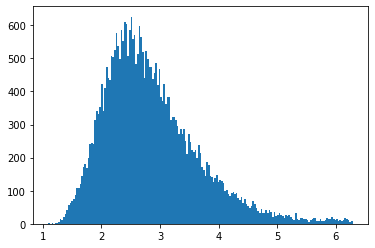
\includegraphics[width=.5\linewidth]{durations}
		\caption{Duration distribution histogram of a subset of speeches}
	\end{figure}
	
	
	
	\section{Data preprocessing}
	\subsection{Data selection by duration}
	We intend to zero pad the data in order to make the samples the same length. To reduce the number of zeroes, we only use the $n$ samples that are closest to each other in duration. This way, we decrease the number of training samples, but hopefully, the efficiency of our network will be much better.
	
	\subsection{Zero padding}
	Our network architecture only supports samples of the same length. To fulfill this constraint, we add zeroes to the end of each recording. The number of necessary zeroes is calculated from the difference between the longest and the current sample.
	
	
	\begin{figure}[H]
		\centering
		\begin{subfigure}{.5\textwidth}
			\centering
			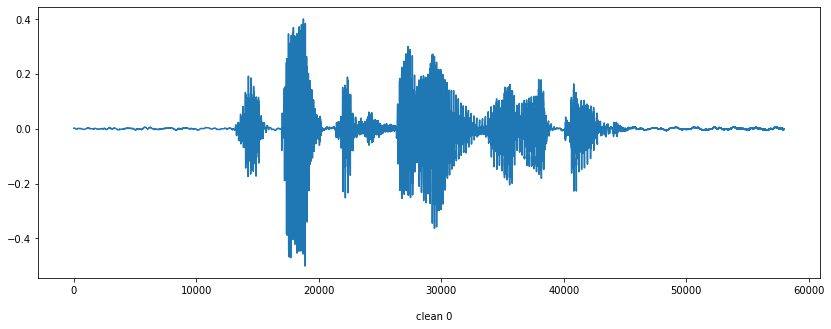
\includegraphics[width=.8\linewidth]{wave_clean}
			\caption{clean}
			\label{fig:wave_clean}
		\end{subfigure}%
		\begin{subfigure}{.5\textwidth}
			\centering
			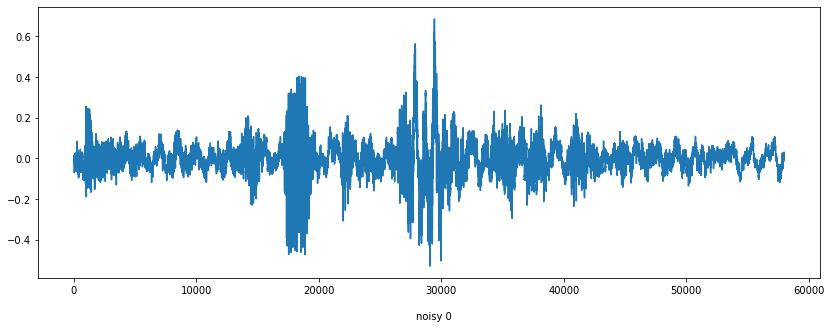
\includegraphics[width=.8\linewidth]{wave_noisy}
			\caption{noisy}
			\label{fig:wave_noisy}
		\end{subfigure}
		\caption{An example clean-noisy pair}
		\label{fig:test}
		
		\begin{subfigure}{.5\textwidth}
			\centering
			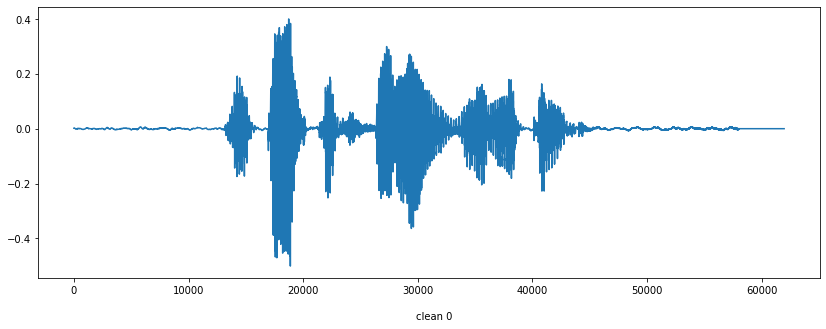
\includegraphics[width=.8\linewidth]{wave_clean_padded}
			\caption{clean}
			\label{fig:wave_clean_padded}
		\end{subfigure}%
		\begin{subfigure}{.5\textwidth}
			\centering
			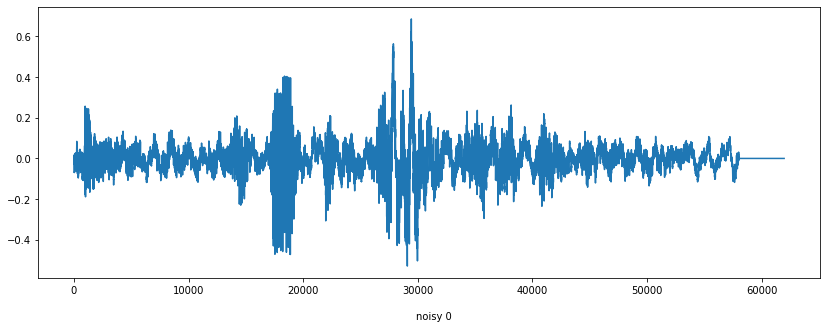
\includegraphics[width=.8\linewidth]{wave_noisy_padded}
			\caption{noisy}
			\label{fig:wave_noisy_padded}
		\end{subfigure}
		\caption{An example clean-noisy pair after zero padding}
		\label{fig:test}
	\end{figure}

	\subsection{\boldmath$\mu$-law transformation}
	To make future computations faster we, reduce the samples to 8 bit with $\mu$-law transformation.
	
	\begin{figure}[H]
		\centering
		\begin{subfigure}{.5\textwidth}
			\centering
			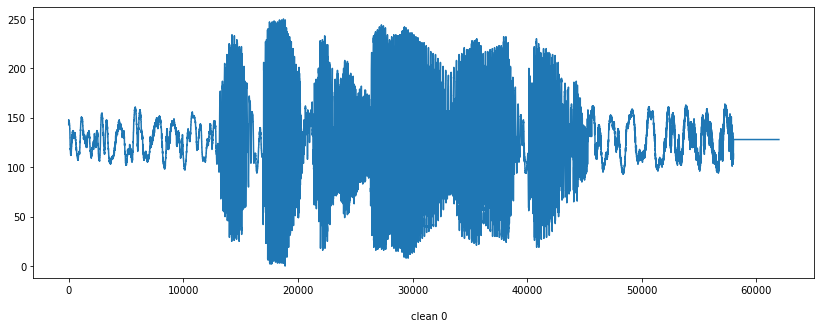
\includegraphics[width=.8\linewidth]{wave_clean_padded_mulaw}
			\caption{clean}
			\label{fig:wave_clean_padded_mulaw}
		\end{subfigure}%
		\begin{subfigure}{.5\textwidth}
			\centering
			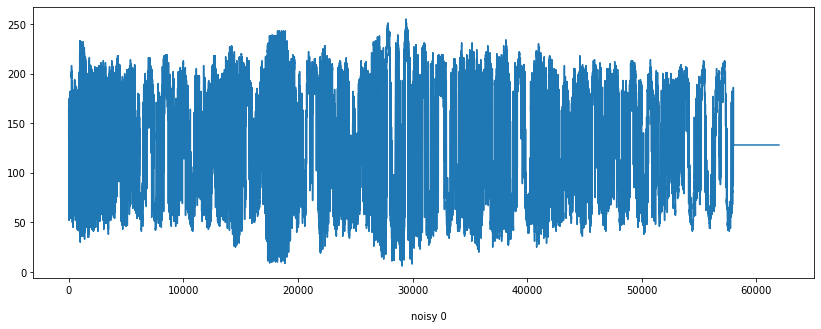
\includegraphics[width=.8\linewidth]{wave_noisy_padded_mulaw}
			\caption{noisy}
			\label{fig:wave_noisy_padded_mulaw}
		\end{subfigure}
		\caption{An example clean-noisy pair after padding and $\mu$-law transformation}
		\label{fig:test}
	\end{figure}
	
	
	
	\newpage
	\printbibliography
	
	
\end{document}
